\documentclass[12pt]{article}
\usepackage{hyperref}
\usepackage{listings}
\usepackage[margin=1in]{geometry}
\usepackage{enumitem}
\usepackage{multicol}
\usepackage{array}
\usepackage{titlesec}
\usepackage{helvet}
\renewcommand{\familydefault}{\sfdefault}
\usepackage{amsmath}     % For math equations
\usepackage{amssymb}     % For advanced math symbols
\usepackage{amsfonts} % For math fonts
\usepackage{gvv}
\usepackage{esint}
\usepackage[utf8]{inputenc}
\usepackage{graphicx}
\usepackage{pgfplots}
\pgfplotsset{compat=1.18}
\titleformat{\section}{\bfseries\large}{\thesection.}{1em}{}
\setlength{\parindent}{0pt}
\setlength{\parskip}{6pt}
\usepackage{multirow}
\usepackage{float}
\usepackage{caption}


\begin{document}
\section*{Problem Statement}
Find the equation of the plane passing through the intersection of the planes 
\begin{align}
\vec{n}_1^\top \vec{x} - c_1 = 0, 
\qquad
\vec{n}_2^\top \vec{x} - c_2 = 0
\end{align}

which is parallel to the $x$-axis, and compute the perpendicular distance of this plane from the $x$-axis.

\section*{Input Data}
\begin{table}[H]
\centering
\begin{tabular}{|c|c|}
\hline
\textbf{Quantity} & \textbf{Value} \\
\hline
$\vec{n}_1$ & $\myvec{1\\1\\1}$ \\
\hline
$c_1$ & $1$ \\
\hline
$\vec{n}_2$ & $\myvec{2\\3\\-1}$ \\
\hline
$c_2$ & $-4$ \\
\hline
$\vec{e}_1$ & $\myvec{1\\0\\0}$ \\
\hline
\end{tabular}
\caption{Input data for the problem}
\label{}
\end{table}


\section*{Solution}

\textbf{Step 1. General plane through the intersection}
\begin{align}
\big(\vec{n}_1 + k \vec{n}_2\big)^\top \vec{x} - \big(c_1 + k c_2\big) &= 0 \\
\vec{n} &= \vec{n}_1 + k \vec{n}_2 \\
c &= c_1 + k c_2
\end{align}

\textbf{Step 2. Condition for parallelism with $x$-axis}
\begin{align}
\vec{e}_1^\top \vec{n} &= 0 \\
\vec{e}_1^\top \vec{n}_1 + k\, \vec{e}_1^\top \vec{n}_2 &= 0 \\
k &= -\frac{\vec{e}_1^\top \vec{n}_1}{\vec{e}_1^\top \vec{n}_2}
\end{align}

\textbf{Step 3. Required plane}
\begin{align}
\vec{n} &= \vec{n}_1 - \frac{\vec{e}_1^\top \vec{n}_1}{\vec{e}_1^\top \vec{n}_2}\,\vec{n}_2 \\
c &= c_1 - \frac{\vec{e}_1^\top \vec{n}_1}{\vec{e}_1^\top \vec{n}_2}\,c_2 \\
\vec{n}^\top \vec{x} &= c
\end{align}

\textbf{Step 4. Distance from the $x$-axis}

Let a point on the $x$-axis be
\begin{align}
\vec{P} &= t \vec{e}_1
\end{align}
The perpendicular distance is
\begin{align}
d &= \frac{\left|\vec{n}^\top \vec{P} - c\right|}{\|\vec{n}\|} \\
&= \frac{|c|}{\|\vec{n}\|}, \quad \text{since } \vec{n}^\top \vec{e}_1 = 0
\end{align}

\textbf{Step 5. Substitution of values}
\begin{align}
\vec{e}_1^\top \vec{n}_1 &= 1, & \vec{e}_1^\top \vec{n}_2 &= 2 \\
k &= -\tfrac{1}{2} \\
\vec{n} &= \vec{n}_1 - \tfrac{1}{2}\vec{n}_2 = \myvec{0\\ -\tfrac12 \\ \tfrac32} \\
c &= c_1 - \tfrac{1}{2} c_2 = 3
\end{align}

Norm:
\begin{align}
\|\vec{n}\|^2 &= \vec{n}_1^\top \vec{n}_1 
- \vec{n}_1^\top \vec{n}_2 
+ \tfrac{1}{4}\vec{n}_2^\top \vec{n}_2 \\
&= 3 - 4 + \tfrac{1}{4}(14) = \tfrac{5}{2} \\
\|\vec{n}\| &= \tfrac{\sqrt{10}}{2}
\end{align}

\textbf{Final Results}
\begin{align}
\text{Equation of Plane:} \quad 
&\big(\vec{n}_1 - \tfrac{1}{2}\vec{n}_2\big)^\top \vec{x} = c_1 - \tfrac{1}{2}c_2 \\
&\Longrightarrow \myvec{0 & -\tfrac12 & \tfrac32}\vec{x} = 3 \\[6pt]
\text{Distance from $x$-axis:} \quad 
&d = \frac{|3|}{\sqrt{10}/2} = \frac{6}{\sqrt{10}} = \frac{3\sqrt{10}}{5}
\end{align}

\begin{figure}[H]
    \centering
    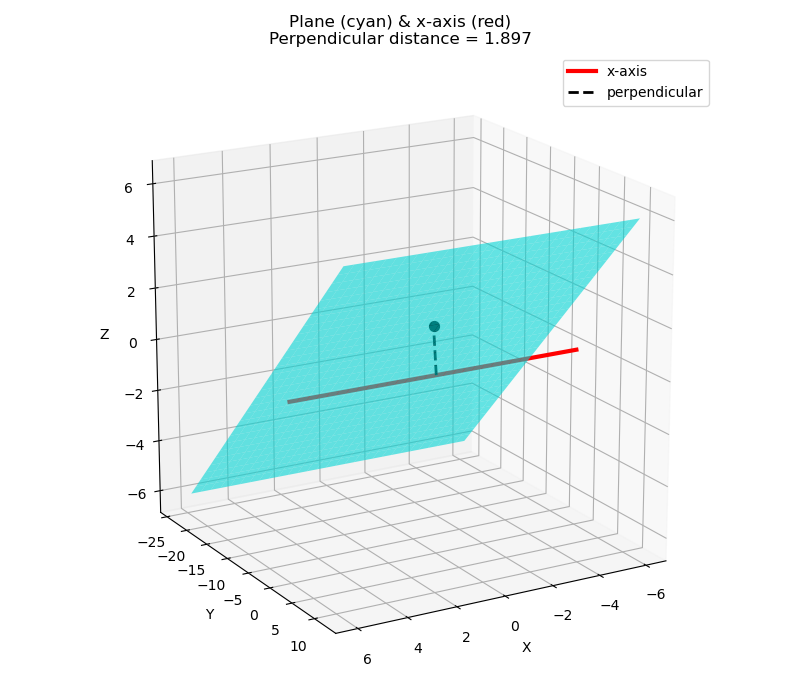
\includegraphics[width=0.9\columnwidth]{figs/plane.png}
    \caption{}
    \label{fig:placeholder}
\end{figure}


\end{document}
